\documentclass{article}
\usepackage{enumitem}

\newlist{FR}{enumerate}{1}
\setlist[FR]{label=FR-\arabic*:}


\renewcommand{\labelenumii}{\theenumii}
\renewcommand{\theenumii}{\theenumi.\arabic{enumii}.}

\usepackage{graphicx}
\graphicspath{{Figures/}}


\title{Software Requirements Specification}
\date{24 February 2017}
\author{Team Dodger}

\begin{document}
	\pagenumbering{gobble}
	\maketitle
	\newpage
	\tableofcontents
	\newpage
	\pagenumbering{arabic}
	
	\section{Introduction}
	The software requirements specification (SRS) should aptly outline the functional requirements of the system to ensure that a third party could develop the functionality to a required degree without further input. Thus, the functional requirements should be precise and extensive to eliminate deviation from the system’s goals.
	
	\subsection{Purpose}
	The intended audience of the application includes students of the University of Pretoria, the staff and simple visitors. NavUP can be used by new students who do not know their way around campuses yet, or simply by staff members who want to avoid clustered pathways. It is a tool that will help optimise campus navigation and reduce travel time from one destination to the other.
	
	\subsection{Scope}
	The NavUP system will help users to navigate campuses by allowing users to choose destinations, locate their current location, set up the appropriate path by taking into account human congestion and visually representing said path for the user to follow.
	NavUP will have a notifications system that will tell the user of events he/she might be interested in. An achievements system will also be in place to award users for walking certain distances or visiting certain locations.  NavUP also hopes to incorporate locations with access for the disabled into its maps for those that are in need of such features. It will have a timetable feature that will allow users to create personalised timetables which the system could then use to help them get where they need to when they need to. The system will work offline but will lose some of its online features such as notifications for user interests. Users will also be able to broadcast their location so that others can see them on their maps.
	
	\subsection{Definitions, Acronyms and Abbreviations}
	
	\begin{figure}[h!]
		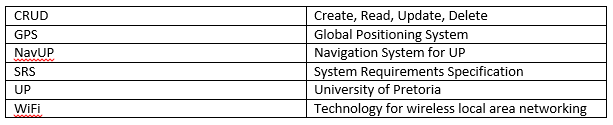
\includegraphics[scale=1]{Descriptions.PNG}
	\end{figure}
	
	\subsection{References}
	\subsection{Overview}
	The SRS will help give a detailed representation of the functional requirements and how the elements of the system interact with eachother to achieve NavUp's purpose. 
	
	\section{Overall Description}
	\subsection{Product Perspective}
	\subsection{Product Function}
	\subsection{User Characteristics}
	\subsection{Constraints}
	This section describes restrictions on the options that are available when developing the application within feasable regions.
		\begin{itemize}
			\item Connections are limited to different types of networks at different locations. GPS cannot be used within buildings and some buildings lack a strong Wi-Fi signal. Mobile networks may also switch to EDGE in some buildings where faster connections aren't available.
			\item Application is initially constrained to Android and iOS only.
			\item Application is designed for approximately 30000 users at any given time which can be seen as a constraint on the number of active users the system can handle.
			\item The application can experience lengthy response times given that there is a constraint resulting from the capacity of the databases.\newline
		\end{itemize}
	
	\subsection{Assumptions and Dependencies}
	
	\section{Specific Requirements}
	This section expands on the functional requirements of the system. It gives a detailed 	description of the system and all of its use cases.
	
	\subsection{External Interface Requirements}
	This section provides a detailed description for each interface that composes the system along with other relevant information.
		\subsubsection{User Interface}
		\begin{itemize}
		\item The user interface should initially be a login screen for first time users or logged out users. This login screen will also have the option for new users to register.
		\item Users should then be able to type in their preferred destination or search via an advanced search method to find a number of different places based on their search criteria.
		\item A results page will be in the form of a visual map which can be used interactively by the user to view his/her route clearly or to view other places of interest along the way.
		\item A settings page will be available for users to tweak the application to their needs as well as to update personal settings.\newline
		\end{itemize}
		
		\subsubsection{Hardware Interface}
		\begin{itemize}
		\item Abstract interface via application and database infrastructure not visible to user.\newline
		\end{itemize}
		
		\subsubsection{Software Interface}
		\begin{itemize}
		\item Application and GPS application communicate in order to receive geographical information. 			\item Application and database communicate in order to receive information about classes and desired locations.\newline
		\end{itemize}
		
		\subsubsection{Communication Interface}
		\begin{itemize}
		\item No specific interface implemented. Communication is left to the underlying operating system of the application and portal/database.\newline
		\end{itemize}
		
	
	\subsection{Functional Requirements}
	This section includes all functional requirements in detail. It includes all use case diagrams, Actor-System interaction diagrams as well as a traceability matrix.	
	\subsubsection{High Level Requirements}
	\begin{FR}
		\item The system should have basic navigation functionality 
		\item The system should be able to provide and visualise information related to pedestrian traffic
		\item The system should be able to push new information to users based on their preferences and interests
		\item The system should integrate various activities that use location and movement
		\item The system should provide functionality to create, read, update and delete users 
		\item The system should allow users to create and manage timetables
		\item The system should allow users to save and share locations
		\item The system should be able to allow users to manage events they are interested in on campus
	\end{FR}
	\subsubsection{Use cases}
	\begin{enumerate}
		\item \underline{Navigation Subsystem}
			
		
	\begin{enumerate}
		\item Get current location
		\begin{enumerate}
			\item \textbf{Description:} The NavUP system must be able to determine a user’s location at any point in time while the user is on the Hatfield campus. The location must be determined regardless of whether the user is indoors or outdoors.
			\item \textbf{Precondition:} The user must have an active account and must be within range of WiFi routers.
			\item \textbf{Postcondition:} The user’s location is determined and displayed.\newline
		\end{enumerate}
		
		\item Search location
		\begin{enumerate}
			\item \textbf{Description:} The NavUP system must provide functionality that enables a user to search for any location (lecture hall, day-house, restaurant) on the Hatfield Campus.
			\item \textbf{Precondition:} The user must have an active account
			\item \textbf{Postcondition:} Matching locations are returned to the user. If no buildings match the search criteria, an appropriate error message is displayed.\newline
		\end{enumerate}
		
		
		\item View location details
		\begin{enumerate}
			\item \textbf{Description:} The NavUP system must allow users to view details related to specific locations. This could include restaurant menus, lecture hall timetable schedules as well as images of the buildings.
			\item \textbf{Precondition:} The user must have an active account and a valid location must be selected on the map.
			\item \textbf{Postcondition:} Relevant location details shown to user.\newline
		\end{enumerate}
		
		\item View places of interest
		\begin{enumerate}
			\item \textbf{Description:} The NavUP system must be able to display places of interests to a user based on their current location. This will include places like restaurants and day-houses that must be displayed in a list form. 
			\item \textbf{Precondition:} The user must have an active account and their current location must be known.  
			\item \textbf{Postcondition:} Relevant places of interest are listed and displayed to the user based on their location.\newline
		\end{enumerate}
		
		\item Navigate to location
		\begin{enumerate}
			\item \textbf{Description:} The NavUP system must be able to provide directions and navigate to a location given the user’s current location as well as a desired destination. The system should calculate the most optimal route by looking at the shortest path as well as pedestrian traffic.
			\item \textbf{Precondition:} The user must have an active account. The user’s current location must be known and the must have specified a destination through the search interface.
			\item \textbf{Postcondition:} The user is provided with directions from their current location to their desired destination.\newline
		\end{enumerate}
		
		\item Show pedestrian traffic
		\begin{enumerate}
			\item \textbf{Description:} The NavUP system must be able to display pedestrian traffic on campus in the form of a heatmap. When navigating to a specified location, the system must show traffic on that specific route. A user should also be able to view an overall heatmap of the campus to see traffic.
			\item \textbf{Precondition:} Users must all have the NavUP app installed and must be registered in order for them to show up on the heatmap.
			\item \textbf{Postcondition:} A heatmap of the campus is displayed. 
		\end{enumerate}
	\end{enumerate}
	\begin{figure}[h!]
		\includegraphics[scale=0.5]{Navigation_Subsystem.png}
		\caption{Navigation Subsystem}	
	\end{figure}
	
	
	\item \underline{Location Management Subsystem}
	\item \underline{User Account Management Subsystem}
	
	
	\item \underline{Entertainment Subsystem}
			\begin{enumerate}
		\item View events
		\begin{enumerate}
			\item \textbf{Description:} The NavUP system must enable users to view all events that are happening around campus in chronological order. The system should suggest events to a user based on their preferences and most visited locations.
			\item \textbf{Precondition:} The user must have an active account and must be logged in.
			\item \textbf{Postcondition:} Various campus-wide events are returned to the user.\newline
		\end{enumerate}
		
		\item Save event
		\begin{enumerate}
			\item \textbf{Description:} The NavUP system must enable users to save events that they are interested so that they can be viewed later.
			\item \textbf{Precondition:} The user must have an active account, must be logged in and there must be events available to save.
			\item \textbf{Postcondition:} An event is saved.\newline
		\end{enumerate}
		
		\item Delete event
		\begin{enumerate}
			\item \textbf{Description:} The NavUP system must enable a user to delete any saved events
			\item \textbf{Precondition:} The user must have an active account, must be logged in and must have saved events
			\item \textbf{Postcondition:} A saved event is deleted .\newline
		\end{enumerate}
	\end{enumerate}
	\begin{figure}[h!]
		\includegraphics[scale=0.5]{Entertainment_Subsystem.png}
		\caption{Navigation Subsystem}	
	\end{figure}	
	
	\item \underline{Achievements Subsystem}
	\item \underline{Administration Subsystem}
	\end{enumerate}
	
	
	\subsection{Performance Requirements}
	Not relevant
	
	\subsection{Design Constraints}
	This section describes restrictions on design alternatives regarding standards and limitations of hardware capabilities.
	\begin{enumerate}
			\item \textbf{Storage space}\newline
			 \textbf{Description:} The amount of storage space required by the application must be within the maximum storage limits of a budget phone to accomodate a range of phones typically used by students.
			\begin{itemize}
			\item \textbf{Maximum:} 90MB
			\item \textbf{Reasonable:} 40MB
			\item \textbf{Optimal:} 10MB.\newline
			\end{itemize}
	
			\item \textbf{Memory usage}\newline
			\textbf{Description:} The amount of RAM used by the application should be a reasonable amount considering that some smartphones only have a capacity of 1GB RAM
			\begin{itemize}
			\item \textbf{Maximum:} 150MB
			\item \textbf{Reasonable:} 90MB
			\item \textbf{Optimal:} 40MB.\newline
			\end{itemize}
	\end{enumerate}
	
	\subsection{Software System Attributes}
	This section describes all quality related requirements of the software system.
	\begin{enumerate}
			\item \textbf{Reliability}\newline
			 \textbf{Description:} The system should return results that are trustable and accurate
			\begin{itemize}
			\item \textbf{Minimum:} 98\% response and accuracy rate
			\item \textbf{Reasonable:} 99\% response and accuracy rate
			\item \textbf{Optimal:} 100\% response and accuracy rate\newline
			\end{itemize}
		
			\item \textbf{Security}\newline
			\textbf{Description:} The system must maintain encryption between system and server so that usernames and passwords remain confidential and database security is not compromised.
			\begin{itemize}
			\item \textbf{Minimum:} 100\% encryption and security rate
			\item \textbf{Reasonable:} 100\% encryption and security rate
			\item \textbf{Optimal:} 100\% encryption and security rate\newline
			\end{itemize}
			
			\item \textbf{Availability}\newline
			\textbf{Description:} The system must be usable at any given time since it will be used by students during the day and possibly visitors for events during the night.
			\begin{itemize}
			\item \textbf{Minimum:} 98\% availability rate
			\item \textbf{Reasonable:} 99\% availability rate
			\item \textbf{Optimal:} 100\% availability rate\newline
			\end{itemize}
			
			\item \textbf{Interoperability}\newline
			\textbf{Description:} The system must have the ability to exchange and use data between the application and database effectively.
			\begin{itemize}
			\item \textbf{Minimum:} 98\% Interoperability rate
			\item \textbf{Reasonable:} 99\% Interoperability rate
			\item \textbf{Optimal:} 100\% Interoperability rate\newline
			\end{itemize}
	\end{enumerate}
	\subsection{Other Requirements}
	Not relevant
\end{document}